\documentclass{LZU}
%\CTEXsetup[format+={\zihao{1}}]{contentname}

\usepackage[backend=biber,gbtverbose=true,
	bibstyle=gbt7714_2005_n,citestyle=gbt7714_2005_n]{biblatex}
\addbibresource{ref.bib}
\renewcommand{\bibfont}{\zihao{5}}

%\title{{兰州大学本科论文格式我也要吧它变成}{一个长标题来看看效果再长一点}{再来一次}}
%\entitle{{Hello WorldHello WorldHello WorldHello}{WorldHello WorldHello WorldHello World}}
\title{{兰州大学本科论文格式我也要吧它变成}{再来一次}}
\entitle{{Hello WorldHello WorldHello WorldHello}}

\pagestyle{fancy}
\begin{document}
\maketitle
\makestatement
\frontmatter
\zhabstract{你好,这个论文的\LaTeX 模板啊,是我根据论文的要求自己写的,凑活着用呗。好像还是不够长,再写两句。写什么呢。}{你好;好的}
\enabstract{
As the first command of the paragraph. This might come in handy when you start a document with body text and not with a sectioning command.

Be careful, however, if you decide to set the indent to zero, then it means you will need a vertical space between paragraphs in order to make them clear. The space between paragraphs is held in , which could be altered in a similar fashion as above. However, this parameter is used elsewhere too, such as in lists, which means you run the risk of making various parts of your document look very untidy by changing this setting. If you want to use the style of having no indentation with a space between paragraphs, use the parskip package, which does this for you, while making adjustments to the spacing of lists and other structures which use paragraph spacing, so they don't get too far apart. If you want both indent and break, use
}{hello, world}
\tableofcontents
\mainmatter
\chapter{中文兰州大学}
%\pagenumbering{arabic}
%\setcounter{page}{1}
\section{第一节}
\subsection{第一条}
粗略地说,是因为复数上不能定义一个序关系使得它与加法和乘法相容。更准确地是复数上不能定义一个全序关系使得复数是一个有序域。很多回答提到复数上能定义偏序关系,但这不是我们想要的序关系,因为它不能与加法和乘法交互。假设复数上能一个全序关系
\begin{figure}[htpb]
    \centering
    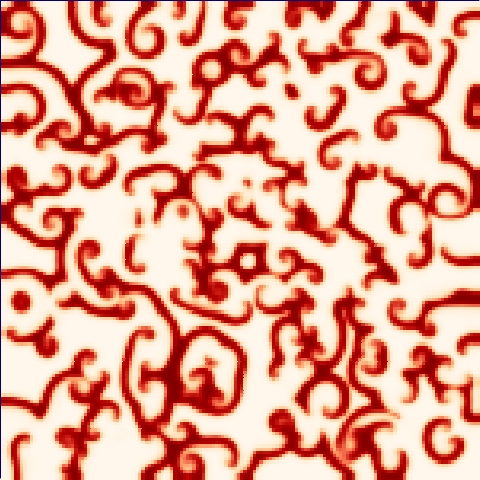
\includegraphics[width=0.6\textwidth]{pic/chaos.png}
    \caption{混沌}
    \label{fig:chaos}
\end{figure}
图图图图图图图图图图图图图图图图图图图图图图图图图图图图图图图图图图图图图图图图图图图图图图图图图图图图图图图图图图图图图图图图图图图图图图图图图图图图图图图图图图图图图图图图图图图图图图图图图图图图图\footnote{注释}
\section{正文(Contents)}
\subsection{标题}
\begin{itemize}
    \item 正文标题:一级标题为三号字,黑体,加粗,居中,单倍行距,段前 24 磅,段后 18 磅;
    \item 二级标题为四号字,黑体,顶左,单倍行 距,段前 24 磅,段后 6 磅;
    \item 三级标题为小四号字,黑体,首行缩进 2 个汉字符,单倍行距,段前 12 磅,段后 6 磅。 正文:采用小四号字,宋体(英文用 Times New Roman 体,12 磅),两端对齐,段落首行左缩进 2 个汉字符,行距 20 磅,段前段 后 0 磅。
\end{itemize}
\begin{equation}
    E=mc^2
\end{equation}

\subsection{图表}
\subsubsection{图}
图:图名置于图的下方,五号字,宋体,居中,单倍行距,段前 6 磅,段后 12 磅,图序与图名之间空 1 个汉字符。
\subsubsection{图}
表:表名置于表的上方,五号字,宋体,居中,单倍行距,段 前 6 磅,段后 6 磅,表序与表名之间空 1 个汉字符。表下方的注释 为五号字,宋体,居左(英文用 Times New Roman 体 10.5 磅),单倍行距。
\subsubsection{注释}
注释:一般分为页末注(脚注)和篇末注。脚注,宋体, 9 磅(英 文用 Times New Roman,9 磅),左对齐,单倍行距,段前段后 0 磅, 按阿拉伯数字编号,每页须重新编号。\footnote{注释啊注释 footnote}
\subsection{图表}
\subsubsection{图}
图:图名置于图的下方,五号字,宋体,居中,单倍行距,段前 6 磅,段后 12 磅,图序与图名之间空 1 个汉字符。
\subsubsection{图}
表:表名置于表的上方,五号字,宋体,居中,单倍行距,段 前 6 磅,段后 6 磅,表序与表名之间空 1 个汉字符。表下方的注释 为五号字,宋体,居左(英文用 Times New Roman 体 10.5 磅),单倍行距。
\subsubsection{注释}
注释:一般分为页末注(脚注)和篇末注。脚注,宋体, 9 磅(英 文用 Times New Roman,9 磅),左对齐,单倍行距,段前段后 0 磅, 按阿拉伯数字编号,每页须重新编号。\footnote{注释啊注释 footnote}
\chapter{例子}
利用 FitzHugh-Nagumo 模型,验证性的研究了心脏细胞的工作机理。\cite{PhysRevLett.76.1619}通过计算机模拟试着在一矩形区域中生成了行波,螺旋波。通过改变一些参数来初步探索了参数对模拟波状态的影响。最后用行波和螺旋波对时空混沌进行了控制。

\printbibliography[title={参考文献},heading=bibintoc]
\Appendix
图图图图图图图图图图图图图图图图图图图图图图图图图图图图图图图图图图图图图图图图图图图图图图图图图图图图图图图图图图图图图图图图图图图图图图图图图图图图图图图图图图图图图图图图图图图图图图图图图图图图图\footnote{注释}
\Thanks
图图图图图图图图图图图图图图图图图图图图图图图图图图图图图图图图图图图图图图图图图图图图图图图图图图图图图图图图图图图图图图图图图图图图图图图图图图图图图图图图图图图图图图图图图图图图图图图图图图图图图\footnote{注释}
\Grade
\end{document}
